% Options for packages loaded elsewhere
\PassOptionsToPackage{unicode}{hyperref}
\PassOptionsToPackage{hyphens}{url}
%
\documentclass[
]{article}
\usepackage{amsmath,amssymb}
\usepackage{lmodern}
\usepackage{iftex}
\ifPDFTeX
  \usepackage[T1]{fontenc}
  \usepackage[utf8]{inputenc}
  \usepackage{textcomp} % provide euro and other symbols
\else % if luatex or xetex
  \usepackage{unicode-math}
  \defaultfontfeatures{Scale=MatchLowercase}
  \defaultfontfeatures[\rmfamily]{Ligatures=TeX,Scale=1}
\fi
% Use upquote if available, for straight quotes in verbatim environments
\IfFileExists{upquote.sty}{\usepackage{upquote}}{}
\IfFileExists{microtype.sty}{% use microtype if available
  \usepackage[]{microtype}
  \UseMicrotypeSet[protrusion]{basicmath} % disable protrusion for tt fonts
}{}
\makeatletter
\@ifundefined{KOMAClassName}{% if non-KOMA class
  \IfFileExists{parskip.sty}{%
    \usepackage{parskip}
  }{% else
    \setlength{\parindent}{0pt}
    \setlength{\parskip}{6pt plus 2pt minus 1pt}}
}{% if KOMA class
  \KOMAoptions{parskip=half}}
\makeatother
\usepackage{xcolor}
\usepackage[margin=1in]{geometry}
\usepackage{longtable,booktabs,array}
\usepackage{calc} % for calculating minipage widths
% Correct order of tables after \paragraph or \subparagraph
\usepackage{etoolbox}
\makeatletter
\patchcmd\longtable{\par}{\if@noskipsec\mbox{}\fi\par}{}{}
\makeatother
% Allow footnotes in longtable head/foot
\IfFileExists{footnotehyper.sty}{\usepackage{footnotehyper}}{\usepackage{footnote}}
\makesavenoteenv{longtable}
\usepackage{graphicx}
\makeatletter
\def\maxwidth{\ifdim\Gin@nat@width>\linewidth\linewidth\else\Gin@nat@width\fi}
\def\maxheight{\ifdim\Gin@nat@height>\textheight\textheight\else\Gin@nat@height\fi}
\makeatother
% Scale images if necessary, so that they will not overflow the page
% margins by default, and it is still possible to overwrite the defaults
% using explicit options in \includegraphics[width, height, ...]{}
\setkeys{Gin}{width=\maxwidth,height=\maxheight,keepaspectratio}
% Set default figure placement to htbp
\makeatletter
\def\fps@figure{htbp}
\makeatother
\setlength{\emergencystretch}{3em} % prevent overfull lines
\providecommand{\tightlist}{%
  \setlength{\itemsep}{0pt}\setlength{\parskip}{0pt}}
\setcounter{secnumdepth}{-\maxdimen} % remove section numbering
\ifLuaTeX
  \usepackage{selnolig}  % disable illegal ligatures
\fi
\IfFileExists{bookmark.sty}{\usepackage{bookmark}}{\usepackage{hyperref}}
\IfFileExists{xurl.sty}{\usepackage{xurl}}{} % add URL line breaks if available
\urlstyle{same} % disable monospaced font for URLs
\hypersetup{
  pdftitle={CT\_ANALYSIS},
  pdfauthor={Finn Lobnow},
  hidelinks,
  pdfcreator={LaTeX via pandoc}}

\title{CT\_ANALYSIS}
\author{Finn Lobnow}
\date{2022-07-22}

\begin{document}
\maketitle

\hypertarget{the-isolates}{%
\section{THE ISOLATES}\label{the-isolates}}

\begin{longtable}[]{@{}
  >{\raggedleft\arraybackslash}p{(\columnwidth - 24\tabcolsep) * \real{0.0246}}
  >{\raggedright\arraybackslash}p{(\columnwidth - 24\tabcolsep) * \real{0.0820}}
  >{\raggedright\arraybackslash}p{(\columnwidth - 24\tabcolsep) * \real{0.0984}}
  >{\raggedright\arraybackslash}p{(\columnwidth - 24\tabcolsep) * \real{0.0820}}
  >{\raggedright\arraybackslash}p{(\columnwidth - 24\tabcolsep) * \real{0.0902}}
  >{\raggedright\arraybackslash}p{(\columnwidth - 24\tabcolsep) * \real{0.0574}}
  >{\raggedright\arraybackslash}p{(\columnwidth - 24\tabcolsep) * \real{0.0984}}
  >{\raggedright\arraybackslash}p{(\columnwidth - 24\tabcolsep) * \real{0.1230}}
  >{\raggedright\arraybackslash}p{(\columnwidth - 24\tabcolsep) * \real{0.0574}}
  >{\raggedright\arraybackslash}p{(\columnwidth - 24\tabcolsep) * \real{0.0820}}
  >{\raggedleft\arraybackslash}p{(\columnwidth - 24\tabcolsep) * \real{0.0410}}
  >{\raggedleft\arraybackslash}p{(\columnwidth - 24\tabcolsep) * \real{0.0902}}
  >{\raggedleft\arraybackslash}p{(\columnwidth - 24\tabcolsep) * \real{0.0738}}@{}}
\toprule()
\begin{minipage}[b]{\linewidth}\raggedleft
X.
\end{minipage} & \begin{minipage}[b]{\linewidth}\raggedright
Species
\end{minipage} & \begin{minipage}[b]{\linewidth}\raggedright
Accession
\end{minipage} & \begin{minipage}[b]{\linewidth}\raggedright
Abbr
\end{minipage} & \begin{minipage}[b]{\linewidth}\raggedright
Subspecies
\end{minipage} & \begin{minipage}[b]{\linewidth}\raggedright
Host
\end{minipage} & \begin{minipage}[b]{\linewidth}\raggedright
Isolate
\end{minipage} & \begin{minipage}[b]{\linewidth}\raggedright
Location
\end{minipage} & \begin{minipage}[b]{\linewidth}\raggedright
Region
\end{minipage} & \begin{minipage}[b]{\linewidth}\raggedright
Quality
\end{minipage} & \begin{minipage}[b]{\linewidth}\raggedleft
Year
\end{minipage} & \begin{minipage}[b]{\linewidth}\raggedleft
Longitude
\end{minipage} & \begin{minipage}[b]{\linewidth}\raggedleft
Latitude
\end{minipage} \\
\midrule()
\endhead
1 & C.tyzzeri & unpublished & EUR\_M\_866 & IXb & Mus & AA\_0866 &
Germany & BR & good & 2022 & 13.55580 & 52.92060 \\
2 & C.tyzzeri & unpublished & EUR\_M\_942 & IXb & Mus & AA\_0942 &
Germany & BR & good & 2022 & 13.28390 & 52.95760 \\
3 & C.tyzzeri & unpublished & EUR\_M\_900 & IXb & Mus & AA\_0900 &
Germany & BR & bad & 2022 & 14.08330 & 52.69670 \\
4 & C.tyzzeri & SRR5683558 & USA\_M\_GA & IXb & Mus & UGA55 & USA & GA &
excellent & 2019 & -83.40056 & 33.98009 \\
5 & C.tyzzeri & SRR16934713 & CHN\_M\_GU & IXa & Mus & TYGZ1 & China &
GU & excellent & 2021 & 113.36774 & 23.36025 \\
6 & C.parvum & SRR15694518 & EUR\_H\_CZ & IIa & Human & Czech5 & Czech
Republic & CZ & excellent & 2017 & 14.99937 & 49.60718 \\
7 & C.parvum & SRR15694490 & USA\_H\_OR & IIc & Human & 43801 & USA & OR
& excellent & 2016 & -120.70518 & 43.83910 \\
8 & C.parvum & SRR15694483 & USA\_H\_AL1 & IIc & Human & M1701011662 &
USA & AL & excellent & 2017 & -86.72669 & 32.92584 \\
9 & C.parvum & SRR15694501 & USA\_H\_AL2 & IId & Human & 45175 & USA &
AL & excellent & 2018 & -86.72669 & 32.92584 \\
10 & C.parvum & SRR15694519 & EUR\_C\_CZ & IIa & Cattle & Czech3 & Czech
Republic & CZ & excellent & 2017 & 14.99937 & 49.60718 \\
11 & C.parvum & SRR15694484 & CHN\_C\_GU1 & IId & Cattle & 22973 & China
& GU & excellent & 2019 & 113.36774 & 23.36025 \\
12 & C.parvum & SRR15694495 & CHN\_C\_GU2 & IId & Cattle & 22972 & China
& GU & excellent & 2019 & 113.36774 & 23.36025 \\
13 & C.parvum & SRR15694506 & CHN\_C\_GU3 & IId & Cattle & 22971 & China
& GU & excellent & 2019 & 113.36774 & 23.36025 \\
14 & C.parvum & SRR15694521 & CHN\_C\_SH1 & IId & Cattle & 22207 & China
& SH & excellent & 2015 & 121.47260 & 31.23931 \\
15 & C.parvum & SRR15694522 & CHN\_C\_SH2 & IId & Cattle & 22600 & China
& SH & excellent & 2016 & 121.47260 & 31.23931 \\
16 & C.parvum & SRR15694502 & USA\_C\_WI & IIa & Cattle & NAMHS-861 &
USA & WI & excellent & 2015 & -89.58182 & 44.69938 \\
17 & C.parvum & SRR15694503 & USA\_C\_WA1 & IIa & Cattle & NAMHS-2153 &
USA & WA & excellent & 2015 & -120.15838 & 47.36275 \\
18 & C.parvum & SRR15694504 & USA\_C\_WA2 & IIa & Cattle & NAMHS-1925 &
USA & WA & excellent & 2015 & -120.15838 & 47.36275 \\
\bottomrule()
\end{longtable}

\hypertarget{samples-with-illumina-sequencing-results}{%
\subsection{Samples with Illumina Sequencing
Results}\label{samples-with-illumina-sequencing-results}}

\begin{figure}
\centering
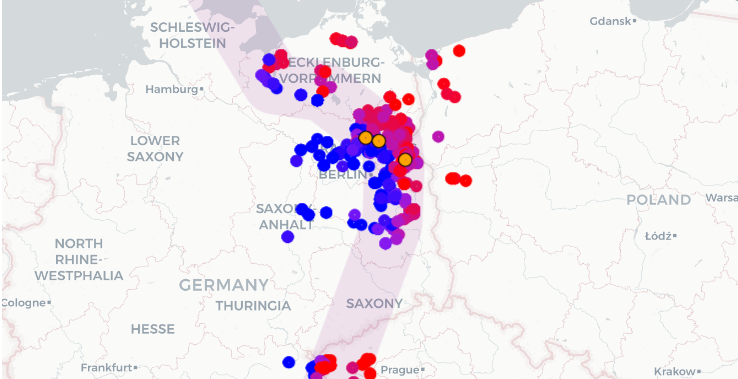
\includegraphics{https://raw.githubusercontent.com/tlobnow/Crypto/main/Genome_Analysis/markdown/illumina.png}
\caption{Illumina Samples}
\end{figure}

\hypertarget{spatial-distribution-of-samples}{%
\subsection{Spatial Distribution of
Samples}\label{spatial-distribution-of-samples}}

\begin{figure}
\centering
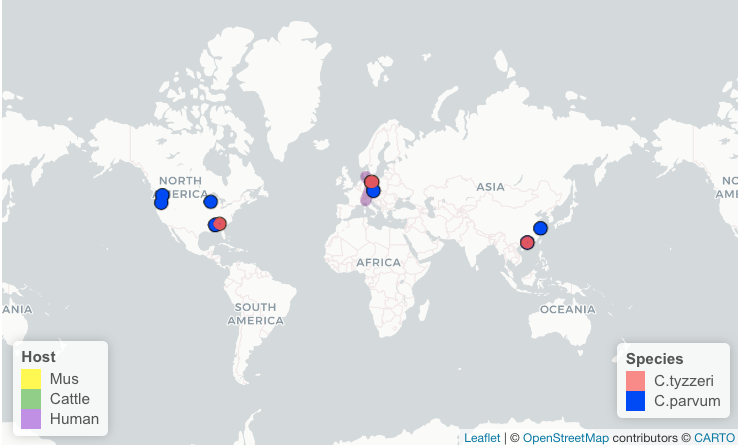
\includegraphics{https://raw.githubusercontent.com/tlobnow/Crypto/main/Genome_Analysis/markdown/sample_spp.png}
\caption{Crypto species distribution}
\end{figure}

\begin{figure}
\centering
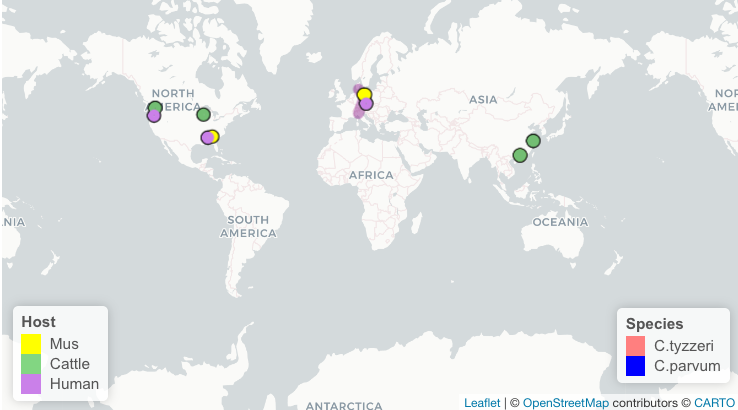
\includegraphics{https://raw.githubusercontent.com/tlobnow/Crypto/main/Genome_Analysis/markdown/samples_host.png}
\caption{Crypto host distribution}
\end{figure}

\hypertarget{workflow}{%
\section{WORKFLOW}\label{workflow}}

\hypertarget{download-data-from-sequence-read-archive-sra}{%
\subsection{Download data from Sequence Read Archive
(SRA)}\label{download-data-from-sequence-read-archive-sra}}

\begin{verbatim}
prefetch SRR*
\end{verbatim}

\hypertarget{split-files}{%
\subsection{Split files}\label{split-files}}

\begin{verbatim}
fasterq-dump *.sra --split-files
\end{verbatim}

\hypertarget{qc-and-trimming}{%
\subsection{QC and trimming}\label{qc-and-trimming}}

--in1 and --in2: specify your files of forward (1) reads and of the
reverse (2) reads.

--out1 and --out2: specify the output files for forward and reverse
reads that are still Paired.

-l 50: this specifies that if a read is shorter than 50 base pairs after
all filters, it should be removed.

-h: specifies name for the html file with plots showing the read quality
before and after filtering

\hypertarget{polyg-tail-trimming}{%
\paragraph{PolyG tail trimming}\label{polyg-tail-trimming}}

This feature removes the polyG tails that arise from lack of signal in
NextSeq/NovaSeq technologies. It is enabled for Nextseq/Novaseq data by
default, and you can specify -g to enable it for any data, or specify -G
to disable it.

\hypertarget{removal-of-adapter-sequences}{%
\paragraph{Removal of adapter
sequences}\label{removal-of-adapter-sequences}}

Adapter trimming is enabled by default, but you can disable it with -A.
Adapter sequences can be automatically detected for both PE/SE data.

\hypertarget{length-filter}{%
\paragraph{Length filter}\label{length-filter}}

Reads below the length threshold (e.g.~due to adapter removal) are
removed. Length filtering is enabled by default. The minimum length
requirement is specified with -l.

\hypertarget{quality-filtering}{%
\paragraph{Quality filtering}\label{quality-filtering}}

Quality filtering is enabled by default, but you can disable it with -Q.
Currently fastp supports filtering by limiting the number of uncalled
(N) bases (-n, Default 5) and the percentage of unqualified bases. To
filter reads by its percentage of unqualified bases, two options should
be provided:

-q : Quality threshold per base required. Default: 15, which means that
a Phred quality score of at least 15 is required

-u : Percent of bases allowed to be below the quality threshold to keep
the read (0\textasciitilde100). Default 40 means 40\% bases can fail the
quality threshold. If more bases fail, the read is removed

\begin{verbatim}
01_fastp.sh

#!/usr/bin/env bash

INDS=($(for i in /SAN/Ctyzzeri/all/fastq/*_1.fastq.gz; do echo $(basename -a -s _1.fastq.gz $i); done))

for IND in ${INDS[@]};
do

    ~/fastp.0.23.1/fastp \
    --in1 /SAN/Ctyzzeri/all/fastq/${IND}_1.fastq.gz \
    --in2 /SAN/Ctyzzeri/all/fastq/${IND}_2.fastq.gz \
    --out1 /SAN/Ctyzzeri/all/results/filteredReads/${IND}.trimmed.R1.fastq.gz \
    --out2 /SAN/Ctyzzeri/all/results/filteredReads/${IND}.trimmed.R2.fastq.gz -l 50 -h /SAN/Ctyzzeri/all/results/qc/filteredReads/${IND}.html &> /SAN/Ctyzzeri/all/results/qc/filteredReads/${IND}.log

done
\end{verbatim}

\hypertarget{indexing-the-reference-sequence}{%
\subsection{Indexing the Reference
Sequence}\label{indexing-the-reference-sequence}}

\begin{verbatim}
02_bwa_index.sh / 02_samtools_faidx.sh

#!/usr/bin/env bash
bwa index /SAN/Ctyzzeri/all/resources/CryptoDB-57_CtyzzeriUGA55_Genome.fasta

#!/usr/bin/env bash
samtools faidx /SAN/Ctyzzeri/all/resources/*.fasta
\end{verbatim}

\hypertarget{mapping-to-the-reference-genome}{%
\subsection{Mapping to the Reference
Genome}\label{mapping-to-the-reference-genome}}

Using alignment software, we essentially find where in the genome our
reads originate from and then once these reads are aligned, we are able
to either call variants or construct a consensus sequence for our set of
aligned reads.

-M is a standard flag that tells bwa to mark any low quality alignments
(i.e.~split across long distances) as secondary - we need this for
downstream compatability.

-t tells bwa how many threads (cores) on a cluster to use - this
effectively determines its speed.

Following these options, we then specify the reference genome, the
forward reads and the reverse reads. Finally we write the output of the
alignment to a SAM file.

\begin{verbatim}
03_bwa_align.sh

#!/usr/bin/env bash

REF=/SAN/Ctyzzeri/all/resources/CryptoDB-57_CtyzzeriUGA55_Genome.fasta
INDS=($(for i in /SAN/Ctyzzeri/all/results/filteredReads/*R1.fastq.gz; do echo $(basename ${i%.R*}); done))

for IND in ${INDS[@]};
do

    # declare variables
    FORWARD=/SAN/Ctyzzeri/all/results/filteredReads/${IND}.R1.fastq.gz
    REVERSE=/SAN/Ctyzzeri/all/results/filteredReads/${IND}.R2.fastq.gz
    OUTPUT=/SAN/Ctyzzeri/all/results/align/${IND}_sort.bam

    # align and sort
    echo "Aligning $IND with bwa"
    bwa mem -M -t 16 $REF $FORWARD $REVERSE | \
    samtools view -b | \
    samtools sort -T ${IND} > $OUTPUT

done
\end{verbatim}

Alternatively, this can be run in parallel after specification of all
individuals in a list:

\begin{verbatim}
for i in /SAN/Ctyzzeri/all/fastq/*1.fastq.gz; do echo $(basename -a -s _1.fastq.gz $i); done > inds
\end{verbatim}

The script can be run using
\texttt{parallel\ \textquotesingle{}sh\ 03\_parallel\_align.sh\ \{\}\textquotesingle{}\ ::::\ inds}

\begin{verbatim}
03_parallel_align.sh

#!/usr/bin/env bash

# align a single individual
REF=/SAN/Ctyzzeri/all/resources/CryptoDB-57_CtyzzeriUGA55_Genome.fasta

# declare variables
IND=$1

FORWARD=/SAN/Ctyzzeri/all/results/filteredReads/${IND}.trimmed.R1.fastq.gz
REVERSE=/SAN/Ctyzzeri/all/results/filteredReads/${IND}.trimmed.R2.fastq.gz
OUTPUT=/SAN/Ctyzzeri/all/results/align/${IND}_sort.bam

# align and sort
echo "Aligning $IND with bwa"
bwa mem -M -t 16 $REF $FORWARD $REVERSE | \
samtools view -b | \
samtools sort -T ${IND} > $OUTPUT
\end{verbatim}

\hypertarget{removing-duplicates}{%
\subsection{Removing Duplicates}\label{removing-duplicates}}

Finally, we need to remove duplicate reads from the dataset to avoid PCR
duplicates and technical duplicates which inflate our sequencing depth
and give us false certainty in the genotype calls.

\begin{verbatim}
04_markdup.sh

#!/usr/bin/env bash

java -jar /home/finn/picard-tools-1.119/MarkDuplicates.jar \
 REMOVE_DUPLICATES=true \
 ASSUME_SORTED=true VALIDATION_STRINGENCY=SILENT \
 MAX_FILE_HANDLES_FOR_READ_ENDS_MAP=1000 \
 INPUT=/SAN/Ctyzzeri/all/results/align/*.bam \
 OUTPUT=/SAN/Ctyzzeri/all/results/rmd/*.rmd.bam \
 METRICS_FILE=/SAN/Ctyzzeri/all/results/qc/rmd/*.rmd.bam.metrics
\end{verbatim}

\hypertarget{indexing-the-bam-files}{%
\subsubsection{Indexing the BAM files}\label{indexing-the-bam-files}}

\begin{verbatim}
05_samtools_index.sh

#!/usr/bin/env bash

samtools index /SAN/Ctyzzeri/all/results/rmd/*.bam
\end{verbatim}

\hypertarget{variant-calling-with-bcftools}{%
\subsection{Variant calling with
bcftools}\label{variant-calling-with-bcftools}}

To call variants, we will first use the samtools mpileup tool to pileup
our BAM files. What does this mean exactly? Well we will take all reads
at a given position and call variants from the reads covering that
position. We need to do this for all individuals. After performing the
pileup, we than pass the output to bcftools call which will actually
call variants.

For bcftools mpileup:

-a - Annotate the vcf - here we add allelic depth (AD), genotype depth
(DP) and strand bias (SP).

-O - the output type. Here it is u which means we do not compress the
output.

-f - specify the reference genome to call variants against.

For bcftools call:

-f - format fields for the vcf - here they are genotype quality (GQ) and
genotype probability (GP).

-v - output variant sites only - i.e.~ignore non-variant parts of the
reads

-m- use bcftools multiallelic caller

-O- specify the output type, here it is z - i.e.~gzipped (compressed)
vcf

-o output path

\begin{verbatim}
06_mpileup.sh

#!/usr/bin/env bash

REF=/SAN/Ctyzzeri/all/resources/CryptoDB-57_CtyzzeriUGA55_Genome.fasta
OUT=/SAN/Ctyzzeri/all/results/vcf/variants.vcf.gz

bcftools mpileup -a AD,DP,SP -Ou -f $REF \
/SAN/Ctyzzeri/all/results/rmd/*.bam | \
bcftools call -f GQ,GP -m -O z -v --ploidy 1 -o $OUT
\end{verbatim}

\hypertarget{indexing-the-vcf-file}{%
\subsection{indexing the vcf file}\label{indexing-the-vcf-file}}

VCF stands for `variant call format' and is a standard format used for
variant calling and in population genomics. Again a detailed
specification can be found online. It can take a bit of getting used to
but it is widely supported and very useful.

These are the first 11 fields of the vcf and they are always present.
What do they mean?

\begin{itemize}
\tightlist
\item
  CHROM - chromosome or scaffold id from the reference genome
\item
  POS - base pair reference position
\item
  ID - SNP id - blank in this case
\item
  REF- Reference base - A,C,G,T or N. More than one indicates an indel
\item
  ALT - Alternaate base - the alternate base called as a variant
\item
  QUAL - Phred quality score for alternate base call (site not
  individual)
\item
  FILTER - filter status - if PASS then all filters passed
\item
  INFO - additional info on each site - explanation stored in header
\item
  FORMAT- the format for the genotype fields
\end{itemize}

\begin{figure}
\centering
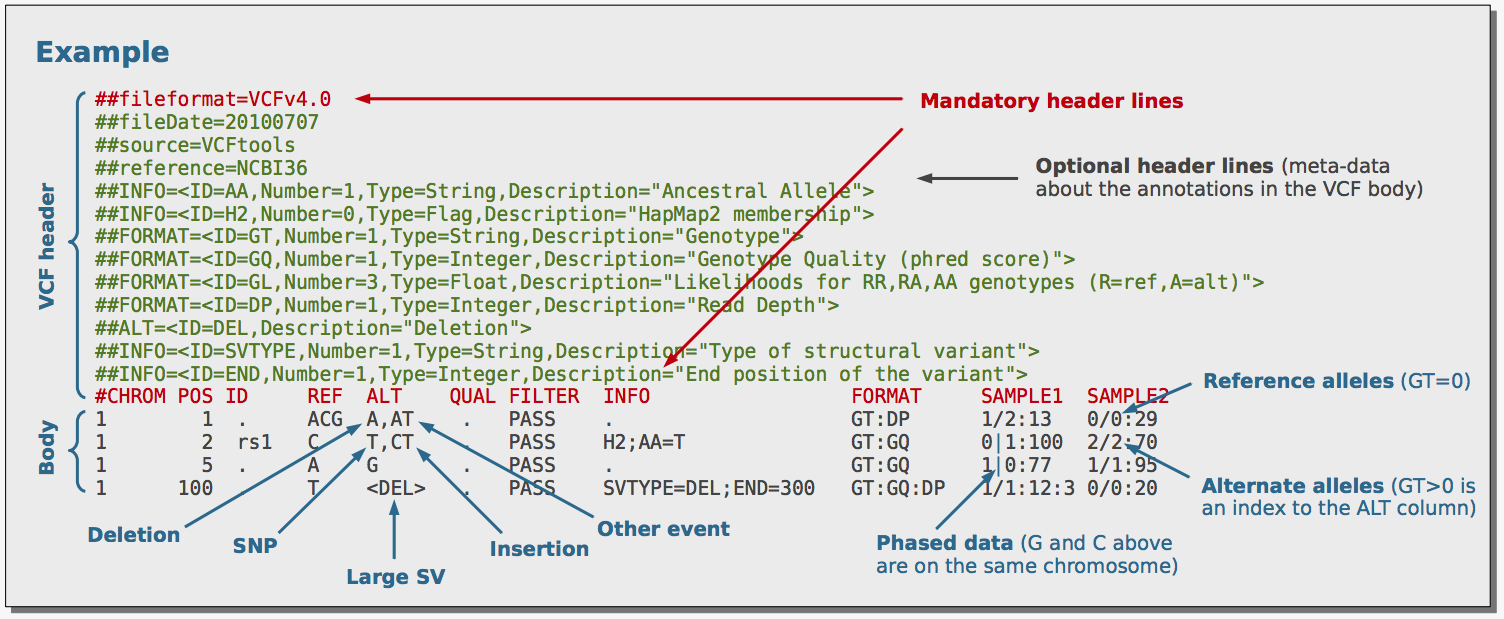
\includegraphics{https://raw.githubusercontent.com/tlobnow/Crypto/main/Genome_Analysis/markdown/vcf_format.png}
\caption{VCF format}
\end{figure}

\begin{verbatim}
07_vcfIndex.sh
bcftools index /SAN/Ctyzzeri/all/results/vcf/variants.vcf.gz
\end{verbatim}

\hypertarget{generating-statistics-on-the-vcf-with-vcftools-local}{%
\subsection{Generating statistics on the VCF with vcftools
(local)}\label{generating-statistics-on-the-vcf-with-vcftools-local}}

In order to generate statistics from our VCF and also actually later
apply filters, we are going to use vcftools, a very useful and fast
program for handling vcf files.

Determining how to set filters on a dataset is a bit of a nightmare - it
is something newcomers (and actually experienced people too) really
struggle with. There also isn't always a clear answer - if you can
justify your actions then there are often multiple solutions to how you
set your filters. What is important is that you get to know your data
and from that determine some sensible thresholds.

Luckily, vcftools makes it possible to easily calculate these
statistics. In this section, we will analyse our VCF in order to get a
sensible idea of how to set such filtering thresholds. The main areas we
will consider are:

\hypertarget{depth}{%
\paragraph{Depth:}\label{depth}}

You should always include a minimum depth filter and ideally also a
maximum depth one too. Minimum depth cutoffs will remove false positive
calls and will ensure higher quality calls too. A maximum cut off is
important because regions with very, very high read depths are likely
repetitive ones mapping to multiple parts of the genome.

\hypertarget{quality}{%
\paragraph{Quality:}\label{quality}}

Genotype quality is also an important filter - essentially you should
not trust any genotype with a Phred score below 20 which suggests a less
than 99\% accuracy.

\hypertarget{minor-allele-frequency}{%
\paragraph{Minor allele frequency:}\label{minor-allele-frequency}}

MAF can cause big problems with SNP calls - and also inflate statistical
estimates downstream. Ideally you want an idea of the distribution of
your allelic frequencies but 0.05 to 0.10 is a reasonable cut-off. You
should keep in mind however that some analyses, particularly demographic
inference can be biased by MAF thresholds.

\hypertarget{missing-data}{%
\paragraph{Missing data:}\label{missing-data}}

How much missing data are you willing to tolerate? It will depend on the
study but typically any site with \textgreater25\% missing data should
be dropped.

For bigger files, it makes sense to generate a vcfrandomsample subset,
but these files are small enough.

The entire script to generate statistics can be looped as follows:

\begin{verbatim}
08_vcfStats.sh

INDS=($(for i in ~/Documents/Github/Crypto/Genome_Analysis/products/vcf/*.vcf.gz; do echo $(basename -a -s *.vcf.gz $i); done))

for IND in ${INDS[@]};
do

    #### Calculate allele frequency
    vcftools --gzvcf ~/Documents/Github/Crypto/Genome_Analysis/products/vcf/${IND} --freq2 --out ~/Documents/Github/Crypto/Genome_Analysis/products/vcftools/${IND}

    #### Calculate mean depth of coverage per individual
    vcftools --gzvcf ~/Documents/Github/Crypto/Genome_Analysis/products/vcf/${IND} --depth --out ~/Documents/Github/Crypto/Genome_Analysis/products/vcftools/${IND}

    #### Calculate mean depth of coverage for  each site
    vcftools --gzvcf ~/Documents/Github/Crypto/Genome_Analysis/products/vcf/${IND} --site-mean-depth --out ~/Documents/Github/Crypto/Genome_Analysis/products/vcftools/${IND}

    #### Calculate the site quality score for each site
    vcftools --gzvcf ~/Documents/Github/Crypto/Genome_Analysis/products/vcf/${IND} --site-quality --out ~/Documents/Github/Crypto/Genome_Analysis/products/vcftools/${IND}

    #### Calculate the proportion of missing data per individual
    vcftools --gzvcf ~/Documents/Github/Crypto/Genome_Analysis/products/vcf/${IND} --missing-indv --out ~/Documents/Github/Crypto/Genome_Analysis/products/vcftools/${IND}

    #### Calculate the propoortion of missing data per site
    vcftools --gzvcf ~/Documents/Github/Crypto/Genome_Analysis/products/vcf/${IND} --missing-site --out ~/Documents/Github/Crypto/Genome_Analysis/products/vcftools/${IND}

    #### Calculate heterozygosity and inbreeding coefficient per individual
    vcftools --gzvcf ~/Documents/Github/Crypto/Genome_Analysis/products/vcf/${IND} --het --out      ~/Documents/Github/Crypto/Genome_Analysis/products/vcftools/${IND}

done
\end{verbatim}

\hypertarget{variant-based-statistics}{%
\subsubsection{VARIANT-BASED
STATISTICS}\label{variant-based-statistics}}

\hypertarget{quality-1}{%
\subparagraph{QUALITY:}\label{quality-1}}

Genotype quality is also an important filter - essentially you should
not trust any genotype with a Phred score below 20 which suggests a less
than 99\% accuracy. We will set the default quality filter to 30, as a
phred score of 30 represents a 1 in 1000 chance that a SNP call is
erroneous.

\begin{itemize}
\tightlist
\item
  QUAL=30
\end{itemize}

\hypertarget{minor-allele-frequency-1}{%
\subparagraph{MINOR ALLELE FREQUENCY:}\label{minor-allele-frequency-1}}

We will take a look at the distribution of allele frequencies. This will
help inform our minor-allele frequency (MAF) thresholds.

The upper bound of the distribution is 0.5, which makes sense because if
MAF was more than this, it wouldn't be the MAF! How do we interpret MAF?
It is an important measure because low MAF alleles may only occur in one
or two individuals. It is possible that some of these low frequency
alleles are in fact unreliable base calls - i.e.~a source of error.

Setting MAF cutoffs is actually not that easy or straightforward. Hard
MAF filtering (i.e.~setting a high threshold) can severely bias
estimation of the site frequency spectrum and cause problems with
demographic analyses. Similarly, an excess of low frequency, `singleton'
SNPs (i.e.~only occurring in one individual) can mean you keep many
uninformative loci in your dataset that make it hard to model things
like population structure.

Usually then, it is best practice to produce one dataset with a good MAF
threshold and keep another without any MAF filtering at all.

\begin{verbatim}
summary(var_freq_05$maf) # Mean = 0.289     --> ?
summary(var_freq_07$maf) # Mean = 0.212     --> ?
summary(var_freq_18$maf) # Mean = 0.235     --> ?
\end{verbatim}

\begin{itemize}
\tightlist
\item
  (MAF=0.1) or (MAF=0.05) \textless- I'm not sure if/how to set this
  filter.
\end{itemize}

\hypertarget{depth-1}{%
\subparagraph{DEPTH:}\label{depth-1}}

\hypertarget{variant-mean-depth}{%
\paragraph{Variant Mean Depth}\label{variant-mean-depth}}

Next we will examine the mean depth for each of our variants. This is
essentially the number of reads that have mapped to this position. The
output we generated with vcftools is the mean of the read depth across
all individuals - it is for both alleles at a position and is not
partitioned between the reference and the alternative.

Variant Depth with xlim(0,150) and ylim(0, 0.025) gives a better idea of
the distribution.

We could set our minimum coverage at the 5 and 95\% quantiles but we
should keep in mind that the more reads that cover a site, the higher
confidence our basecall is. 10x is a good rule of thumb as a minimum
cutoff for read depth, although if we wanted to be conservative, we
could go with 15x.

What is more important here is that we set a good maximum depth cufoff.
As the outliers show, some regions clearly have extremely high coverage
and this likely reflects mapping/assembly errors and also paralogous or
repetitive regions. We want to exclude these as they will bias our
analyses. Usually a good rule of thumb is something the mean depth x 2

\begin{verbatim}
summary(var_depth_05$mean_depth) # Mean = 42.82     x 2 =  85.64
summary(var_depth_07$mean_depth) # Mean = 67.5032   x 2 = 135.01
summary(var_depth_18$mean_depth) # Mean = 80.51647  x 2 = 161.03
\end{verbatim}

\begin{itemize}
\tightlist
\item
  MIN\_DEPTH = 10
\item
  MAX\_DEPTH = 85.64 / 135.01 / 161.03
\end{itemize}

\hypertarget{missingness}{%
\subparagraph{MISSINGNESS:}\label{missingness}}

\hypertarget{variant-missingness}{%
\paragraph{Variant Missingness}\label{variant-missingness}}

Next up we will look at the proportion of missingness at each variant.
This is a measure of how many individuals lack a genotype at a call
site.

The results indicate relatively high missingness, especially among
\emph{C.tyzzeri} samples. One thing to note here is that vcftools
inverts the direction of missigness, so our 10\% threshold means we will
tolerate 90\% missingness. Different datasets will likely have different
missingness profiles. Typically missingness of 75-95\% is used. We will
accept max. 15\% missingness due to the C.tyzzeri dataset (=0.85).

\begin{verbatim}
summary(var_miss_05$fmiss) # Mean = 0.12570     --> MISS=0.85
summary(var_miss_07$fmiss) # Mean = 0.09642     --> MISS=0.90
summary(var_miss_18$fmiss) # Mean = 0.06108     --> MISS=0.90
\end{verbatim}

\begin{itemize}
\tightlist
\item
  MISS = 0.85 / 0.9 / 0.9
\end{itemize}

\hypertarget{individual-based-statistics}{%
\subsubsection{Individual based
statistics}\label{individual-based-statistics}}

As well as a our per variant statistics we generated earlier, we also
calculated some individual metrics too. WE can look at the distribution
of these to get an idea whether some of our individuals have not
sequenced or mapped as well as others. This is good practice to do with
a new dataset. A lot of these statistics can be compared to other
measures generated from the data (i.e.~principal components as a measure
of population structure) to see if they drive any apparent patterns in
the data.

\hypertarget{mean-depth-per-ind}{%
\paragraph{MEAN-DEPTH PER IND:}\label{mean-depth-per-ind}}

Because we are only plotting data for few individuals, the plot looks a
little disjointed. While there is some evidence that some individuals
were sequenced to a higher depth than others, there are no extreme
outliers. So this doesn't suggest any issue with individual sequencing
depth.

\hypertarget{missing-data-per-ind}{%
\paragraph{MISSING DATA PER IND:}\label{missing-data-per-ind}}

Next we will look at the proportion of missing data per individual. This
is very similar to the missing data per site, but here we will focus on
the fmiss column - i.e.~the proportion of missing data.

Again this shows us, the proportion of missing data per individual is
very small indeed. It ranges from 0.01 - 0.6, so we can safely assume
that some of our individuals are sequenced well, while the extreme
values at 0.6 indicate rather bad sequencing that probably arises from
one of the \emph{C.tyzzeri} samples (AA\_0900 I would assume due to
reportedly bad sequencing). We will therefore set a threshold at 0.1.

\hypertarget{heterozygosity-and-inbreeding-coefficient-per-individual}{%
\paragraph{Heterozygosity and inbreeding coefficient per
individual}\label{heterozygosity-and-inbreeding-coefficient-per-individual}}

We cannot assess heterozygosity due to the haploid nature of
\emph{Cryptosporidium} spp.

Technically, computing heterozygosity and the inbreeding coefficient (F)
for each individual can quickly highlight outlier individuals that are
e.g.~inbred (strongly negative F), suffer from high sequencing error
problems or contamination with DNA from another individual leading to
inflated heterozygosity (high F), or PCR duplicates or low read depth
leading to allelic dropout and thus underestimated heterozygosity
(stongly negative F). However, note that here we assume Hardy-Weinberg
equilibrium. If the individuals are not sampled from the same
population, the expected heterozygosity will be overestimated due to the
Wahlund-effect. It may still be worth to compute heterozygosities even
if the samples are from more than one population to check if any of the
individuals stands out which could indicate problems.

\hypertarget{all-statistics-summary}{%
\subsubsection{ALL STATISTICS SUMMARY}\label{all-statistics-summary}}

\includegraphics{CT_ANALYSIS_PDF_comp_files/figure-latex/ALL-STATS-SUMMARY-1.pdf}
\includegraphics{CT_ANALYSIS_PDF_comp_files/figure-latex/ALL-STATS-SUMMARY-2.pdf}
\includegraphics{CT_ANALYSIS_PDF_comp_files/figure-latex/ALL-STATS-SUMMARY-3.pdf}

\hypertarget{filtering-based-on-statistics}{%
\subsection{FILTERING BASED ON
STATISTICS}\label{filtering-based-on-statistics}}

Now we have an idea of how to set out thresholds, we will do just that
and filter for certain attributes:

\begin{itemize}
\item
  --gvcf - input path -- denotes a gzipped vcf file
\item
  --remove-indels - remove all indels (SNPs only)
\item
  --maf - set minor allele frequency - 0.1 here
\item
  --max-missing - set minimum missing data. A little counterintuitive -
  0 is totally missing, 1 is none - missing. Here 0.75 means we will
  tolerate 25\% missing data.
\item
  --minQ - this is just the minimum quality score required for a site to
  pass our filtering threshold. Here we set it to 30.
\item
  --min-meanDP - the minimum mean depth for a site.
\item
  --max-meanDP - the maximum mean depth for a site.
\item
  --minDP - the minimum depth allowed for a genotype - any individual
  failing this threshold is marked as having a missing genotype.
\item
  --maxDP - the maximum depth allowed for a genotype - any individual
  failing this threshold is marked as having a missing genotype.
\item
  --recode - recode the output - necessary to output a vcf
\item
  --stdout - pipe the vcf out to the stdout (easier for file handling)
\end{itemize}

(vcftools is NOT available on Harriet..)

\begin{verbatim}
09_filterVCF.sh

#!/usr/bin/env bash

VCF_IN=~/Desktop/vcf/variants.vcf
VCF_OUT=~/Desktop/vcfFiltered/variants_filtered.vcf.gz

# set filters
MAF=  X
MISS= X
QUAL= X
MIN_DEPTH= X
MAX_DEPTH= X

# perform the filtering with vcftools
vcftools --gzvcf $VCF_IN \
--remove-indels --maf $MAF --max-missing $MISS --minQ $QUAL \
--min-meanDP $MIN_DEPTH --max-meanDP $MAX_DEPTH \
--minDP $MIN_DEPTH --maxDP $MAX_DEPTH --recode --stdout | gzip -c > \
$VCF_OUT
\end{verbatim}

\includegraphics{CT_ANALYSIS_PDF_comp_files/figure-latex/ALL-STATS-SUMMARY-FILTERS-1.pdf}
\includegraphics{CT_ANALYSIS_PDF_comp_files/figure-latex/ALL-STATS-SUMMARY-FILTERS-2.pdf}
\includegraphics{CT_ANALYSIS_PDF_comp_files/figure-latex/ALL-STATS-SUMMARY-FILTERS-3.pdf}

\hypertarget{principal-component-analysis-pca}{%
\subsection{PRINCIPAL COMPONENT ANALYSIS
(PCA)}\label{principal-component-analysis-pca}}

Essentially, PCA aims to identify the main axes of variation in a
dataset with each axis being independent of the next (i.e.~there should
be no correlation between them). The first component summarizes the
major axis variation and the second the next largest and so on, until
cumulatively all the available variation is explained. In the context of
genetic data, PCA summarizes the major axes of variation in allele
frequencies and then produces the coordinates of individuals along these
axes.

\hypertarget{linkage-pruning}{%
\subsubsection{LINKAGE PRUNING}\label{linkage-pruning}}

\hypertarget{linkage-pruning-1}{%
\subsection{Linkage Pruning}\label{linkage-pruning-1}}

One of the major assumptions of PCA is that the data we use is
independent - i.e.~there are no spurious correlations among the measured
variables. This is obviously not the case for most genomic data as
allele frequencies are correlated due to physical linkage and linkage
disequilibrium. So as a first step, we need to prune our data set of
variants that are in linkage.

\begin{itemize}
\item
  --vcf - specified the location of our VCF file.
\item
  --double-id - told plink to duplicate the id of our samples (this is
  because plink typically expects a family and individual id - i.e.~for
  pedigree data - this is not necessary for us.
\item
  --allow-extra-chr - allow additional chromosomes beyond the human
  chromosome set. This is necessary as otherwise plink expects
  chromosomes 1-22 and the human X chromosome.
\item
  --set-missing-var-ids - also necessary to set a variant ID for our
  SNPs. Human and model organisms often have annotated SNP names and so
  plink will look for these. We do not have them so instead we set ours
  to default to chromosome:position which can be achieved in plink by
  setting the option @:\# - see here for more info.
\item
  --indep-pairwise - finally we are actually on the command that
  performs our linkage pruning! The first argument, 50 denotes we have
  set a window of 50 Kb. The second argument, 10 is our window step size
  - meaning we move 10 bp each time we calculate linkage. Finally, we
  set an r2 threshold - i.e.~the threshold of linkage we are willing to
  tolerate. Here we prune any variables that show an r2 of greater than
  0.1.
\item
  --out Produce the prefix for the output data.

  10\_linkagePruning.sh

  VCF=/SAN/Ctyzzeri/all/results/vcfFiltered/*\_samples\_filtered.vcf.gz

  \textasciitilde/plink-1.9/plink\\
  --vcf \$VCF --double-id --allow-extra-chr\\
  --set-missing-var-ids @:\#\$1,\$2\\
  --indep-pairwise 50 10 0.1 --out *\_samples
\end{itemize}

\hypertarget{pca}{%
\subsubsection{PCA}\label{pca}}

We can rerun plink with a few additional arguments to get it to conduct
a PCA.

\begin{itemize}
\item
  --extract - this just lets plink know we want to extract only these
  positions from our VCF - in other words, the analysis will only be
  conducted on these.
\item
  --make-bed - this is necessary to write out some additional files for
  another type of population structure analysis - a model based approach
  with admixture.
\item
  --pca - fairly self explanatory, this tells plink to calculate a
  principal components analysis.
\end{itemize}

PCA output:

\begin{itemize}
\item
  cichlids.eigenval - the eigenvalues from our analysis
\item
  cichlids.eigenvec- the eigenvectors from our analysis
\end{itemize}

Plink binary output:

\begin{itemize}
\item
  cichlids.bed - the cichlids bed file - this is a binary file necessary
  for admixture analysis. It is essentially the genotypes of the pruned
  dataset recoded as 1s and 0s.
\item
  cichlids.bim - a map file (i.e.~information file) of the variants
  contained in the bed file.
\item
  cichlids.fam - a map file for the individuals contained in the bed
  file.

  11\_pca.sh

  \#!/usr/bin/env bash

  INDS=(\$(for i in
  /SAN/Ctyzzeri/all/results/vcfFiltered/*\_filtered.vcf.gz; do echo
  \$(basename -a -s \_filtered.vcf.gz \$i); done))

  for IND in \$\{INDS{[}@{]}\}; do

\begin{verbatim}
  ~/plink-1.9/plink \
  --vcf /SAN/Ctyzzeri/all/results/vcfFiltered/15_samples_filtered.vcf.gz --double-id --allow-extra-chr \
  --set-missing-var-ids @:#\$1,\$2 \
  --extract /SAN/Ctyzzeri/all/results/pcaFiltered/15_samples.prune.in  \
  --make-bed --pca --out /SAN/Ctyzzeri/all/results/pcaFiltered/15_samples
\end{verbatim}

  done
\end{itemize}

First we will plot the eigenvalues. It is quite straightforward to
translate these into percentage variance explained (although note, you
could just plot these raw if you wished). Let's take a look at the the
bar plot showing the percentage of variance each principal component
explains.

\hypertarget{c.tyzzeri-ssp.-n5}{%
\paragraph{C.TYZZERI SSP. (n=5)}\label{c.tyzzeri-ssp.-n5}}

set filters:

\begin{itemize}
\tightlist
\item
  QUAL = 30
\item
  MAF = 0.1
\item
  MISS = 0.85
\item
  MIN\_DEPTH = 10
\item
  MAX\_DEPTH = 2*42.82
\end{itemize}

\begin{verbatim}
##   PC          pve
## 1  1 5.523559e+01
## 2  2 2.740809e+01
## 3  3 1.153670e+01
## 4  4 5.819619e+00
## 5  5 1.110220e-14
\end{verbatim}

\begin{verbatim}
## [1]  55.23559  82.64368  94.18038 100.00000 100.00000
\end{verbatim}

\includegraphics{CT_ANALYSIS_PDF_comp_files/figure-latex/tyz-pca-1.pdf}
\includegraphics{CT_ANALYSIS_PDF_comp_files/figure-latex/tyz-pca-2.pdf}

\hypertarget{tyz-par-hom-pca-n-7-filtered-based-on-statistics-stats---new--}{%
\paragraph{TYZ-PAR-HOM PCA (n = 7) filtered based on statistics (STATS)
- new
-}\label{tyz-par-hom-pca-n-7-filtered-based-on-statistics-stats---new--}}

set filters:

\begin{itemize}
\tightlist
\item
  QUAL = 30
\item
  MAF = 0.1
\item
  MISS = 0.9
\item
  MIN\_DEPTH = 10
\item
  MAX\_DEPTH = 2*67.5032
\end{itemize}

\begin{verbatim}
##   PC       pve
## 1  1 44.614246
## 2  2 23.711121
## 3  3 15.957667
## 4  4  9.845508
## 5  5  6.373428
## 6  6  2.706563
## 7  7 -3.208533
\end{verbatim}

\begin{verbatim}
## [1]  44.61425  68.32537  84.28303  94.12854 100.50197 103.20853 100.00000
\end{verbatim}

\includegraphics{CT_ANALYSIS_PDF_comp_files/figure-latex/7_samples-stats-new-1.pdf}
\includegraphics{CT_ANALYSIS_PDF_comp_files/figure-latex/7_samples-stats-new-2.pdf}

\hypertarget{tyz-par-pca-n-7-filtered-based-on-statistics-stats---old--}{%
\paragraph{TYZ-PAR-PCA (n = 7) filtered based on statistics (STATS) -
old
-}\label{tyz-par-pca-n-7-filtered-based-on-statistics-stats---old--}}

set filters: MAF=0.05 MISS=0.90 QUAL=30 MIN\_DEPTH=10 MAX\_DEPTH=50

\begin{verbatim}
##   PC       pve
## 1  1 36.023347
## 2  2 23.768769
## 3  3 17.840759
## 4  4 14.314135
## 5  5  7.545572
## 6  6  3.121628
## 7  7 -2.614211
\end{verbatim}

\begin{verbatim}
## [1]  36.02335  59.79212  77.63288  91.94701  99.49258 102.61421 100.00000
\end{verbatim}

\includegraphics{CT_ANALYSIS_PDF_comp_files/figure-latex/7_samples-stats-old-1.pdf}
\includegraphics{CT_ANALYSIS_PDF_comp_files/figure-latex/7_samples-stats-old-2.pdf}

\hypertarget{tyzzeri-vs.-parvum-n-18}{%
\paragraph{TYZZERI VS. PARVUM (n = 18)}\label{tyzzeri-vs.-parvum-n-18}}

set filters:

\begin{itemize}
\tightlist
\item
  QUAL = 30
\item
  MAF = 0.1
\item
  MISS = 0.9
\item
  MIN\_DEPTH = 10
\item
  MAX\_DEPTH = 2*80.51647
\end{itemize}

\begin{verbatim}
##    PC         pve
## 1   1 47.25446176
## 2   2 19.44401083
## 3   3 15.69646808
## 4   4  6.92581110
## 5   5  4.19130438
## 6   6  3.14121741
## 7   7  2.71866689
## 8   8  1.17385133
## 9   9  0.86905809
## 10 10  0.66560409
## 11 11  0.38748094
## 12 12  0.21926286
## 13 13  0.20130768
## 14 14  0.06817536
## 15 15 -0.01918241
## 16 16 -0.04349182
## 17 17 -0.31704581
## 18 18 -2.57696078
\end{verbatim}

\begin{verbatim}
##  [1]  47.25446  66.69847  82.39494  89.32075  93.51206  96.65327  99.37194
##  [8] 100.54579 101.41485 102.08045 102.46793 102.68720 102.88851 102.95668
## [15] 102.93750 102.89401 102.57696 100.00000
\end{verbatim}

\includegraphics{CT_ANALYSIS_PDF_comp_files/figure-latex/18_samples-stats-1.pdf}
\includegraphics{CT_ANALYSIS_PDF_comp_files/figure-latex/18_samples-stats-2.pdf}

\hypertarget{looking-at-pc2-and-pc3-in-multi-species-pcas-n-7-and-n-18}{%
\subsection{Looking at PC2 and PC3 in multi-species PCAs (n = 7) and (n
= 18)}\label{looking-at-pc2-and-pc3-in-multi-species-pcas-n-7-and-n-18}}

\hypertarget{tyz-par-hom-pca-n-7---new--}{%
\paragraph{TYZ-PAR-HOM PCA (n = 7) - new
-}\label{tyz-par-hom-pca-n-7---new--}}

set filters:

\begin{itemize}
\tightlist
\item
  QUAL = 30
\item
  MAF = 0.1
\item
  MISS = 0.9
\item
  MIN\_DEPTH = 10
\item
  MAX\_DEPTH = 2*67.5032
\end{itemize}

\includegraphics{CT_ANALYSIS_PDF_comp_files/figure-latex/7_samples-stats-new-PC23-1.pdf}
\includegraphics{CT_ANALYSIS_PDF_comp_files/figure-latex/7_samples-stats-new-PC23-2.pdf}

\hypertarget{tyz-par-pca-n-7-filtered-based-on-statistics-stats---old---1}{%
\paragraph{TYZ-PAR-PCA (n = 7) filtered based on statistics (STATS) -
old
-}\label{tyz-par-pca-n-7-filtered-based-on-statistics-stats---old---1}}

set filters: MAF=0.05 MISS=0.90 QUAL=30 MIN\_DEPTH=10 MAX\_DEPTH=50

\includegraphics{CT_ANALYSIS_PDF_comp_files/figure-latex/7_samples-stats-old-PC23-1.pdf}
\includegraphics{CT_ANALYSIS_PDF_comp_files/figure-latex/7_samples-stats-old-PC23-2.pdf}

\hypertarget{tyzzeri-vs.-parvum-n-18-1}{%
\paragraph{TYZZERI VS. PARVUM (n =
18)}\label{tyzzeri-vs.-parvum-n-18-1}}

set filters:

\begin{itemize}
\tightlist
\item
  QUAL = 30
\item
  MAF = 0.1
\item
  MISS = 0.9
\item
  MIN\_DEPTH = 10
\item
  MAX\_DEPTH = 2*80.51647
\end{itemize}

\includegraphics{CT_ANALYSIS_PDF_comp_files/figure-latex/18_samples-stats-PC23-1.pdf}
\includegraphics{CT_ANALYSIS_PDF_comp_files/figure-latex/18_samples-stats-PC23-2.pdf}

\end{document}
